\chapter{Use case diagram}

Figure \ref{ucd} of this Appendix contains the use case diagram. All use-cases described in Appendix B are included in this diagram. The following abbreviations are used:
\begin{description}
\item[C.D.] Concentration Distribution.
\item[M.P.] Mixing Protocol.
\item[M.R.] Mixing Run.
\end{description}

Furthermore, solid arrows represent the \emph{Preceeds} relationship, and dashed arrows represent the \emph{Uses} relationship.

\begin{figure}[h!]
\begin{center}
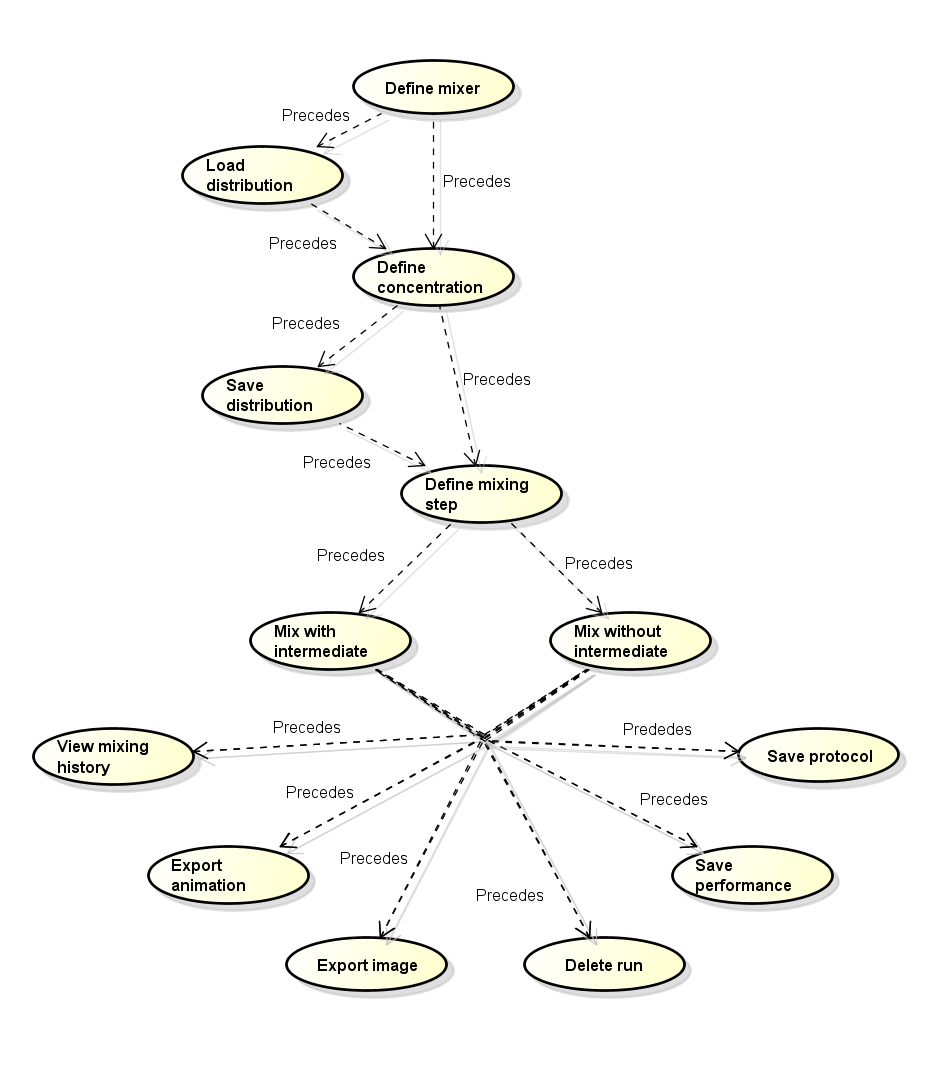
\includegraphics[keepaspectratio=true,width=800 pt,height=508 pt]{UseCaseDiagram.png}\captionof{figure}{Use Case Diagram including all the use cases described in Appendix B.\label{ucd}}
\end{center}
\end{figure}
